
	\documentclass[oneside]{VUMIFPSkursinis}
\usepackage{algorithmicx}
\usepackage{algorithm}
\usepackage{algpseudocode}
\usepackage{amsfonts}
\usepackage{float}
\usepackage{amsmath}
\usepackage{bm}
\usepackage{caption}
\usepackage{color}
\usepackage{float}
\usepackage{graphicx}
\usepackage{listings}
\usepackage{subfig}
\usepackage{wrapfig}
\usepackage[%  
    colorlinks=true,
    linkcolor=black
]{hyperref}
\university{Vilniaus universitetas}
\faculty{Matematikos ir informatikos fakultetas}
\department{Programų sistemų katedra}
\papertype{Laboratorinis darbas I}
\title{Automatinė ūkio valdymo sistema}
\titleineng{Automatic farm management system}
\status{2 kurso 3 grupės studentai}
\author{Matas Savickis}
\secondauthor{Justas Tvarijonas}  
\thirdauthor{Greta Pyrantaitė}   
\fourthauthor{Rytautas Kvašinskas}
\supervisor{Karolis Petrauskas, Doc., Dr.}
\date{Vilnius – \the\year}

% Nustatymai
%\setmainfont{Palemonas}   % Pakeisti teksto šriftą į Palemonas (turi būti įdiegtas sistemoje)
\bibliography{bibliografija}

\begin{document}
\maketitle

\tableofcontents


\centering	
\sectionnonum{Įvadas}
Automatinė ūkio valdymo sistema (toliau - Auto ūkis) yra programa, leidžianti ūkininkui valdyti jo ūkį skaitmeniniu būdu. Auto ūkis leidžia registruoti gyvūnus ir stebėti kiekvieno jų bioparametrus (kraujo spaudimą, svorį, sveikatą) bei matyti ūkio technikos judėjimą po žemės plotą. Taip pat sistema vartotojui leidžia sekti dirvos parametrus (drėgmę, pH lygį), oro prognozes ir gyvūnų ligų paplitimą aplinkinėse teritorijose. Auto ūkis padeda ir su verslo valdymu: nesunkiai galima samdyti darbuotojus, atlikti buhalterinę apyskaitą, stebėti rinkos kainas ir apskaičiuoti bei numatyti galimą pelną. Iškilus nelaimei per Auto ūkio sistemą galima greitai iškviesti greitąją pagalbą, policiją, gaisrinę ar saugos tarnybą. Orų prognozės yra paimtos iš www.gismeteo.lt. Pagrindinė sistemos inovacija yra tai, kad, kai sistema yra pilnai įdiegta, darbuotojų skaičius, reikalingas palaikyti ūkį, tampa minimalus. Kadangi ūkio technika būtų valdoma automatiškai, vairuotojų ir derliaus nurinkėjų nereiktų. Gyvūnų sekimas yra įgyvendinamas mikro kontrolerio su Arduino pagalba. Šis kontroleris nedidelis ir lengvai pritaikomas visokio pobūdžio darbams. Jį, kartu su WiFi moduliu, sistema naudoja gauti gyvūno lokaciją per Google Maps,- taip pasiklydę ar pavogti gyvūnai būtų greitai surandami ir grąžinami. Žemės laistymas ir tręšimas taip pat būtų automatizuotas: parametrai gaunami per Arduino detektorius, kurie pagal pasikeitusią dirvos kompoziciją nusprendžia, ko trūksta žemei, ir aktyvuoja laistymo ir tręšimo sistemas. Darbuotojų samdymas yra įgyvendintas per darbo biržos puslapį, kur greitai ir nesunkiai galimą įdėti skelbimą arba surasti darbuotoją. Buhalterija yra tvarkoma naudojantis nemokama buhalterijos programa Wave Accounting, kuri yra implementuota į Auto ūkį.  Auto ūkio sistema yra parašyta JAVA kalba - tai leidžia programą paleisti ant bet kurios operacinės sistemos. Ateityje numatoma galimybė programą perkelti į išmaniuosius telefonus. Sistema buvo projektuojama pasitelkiant www.planttext.com ir www.draw.io funkcionalumą.

\section{Perprojektuotos sistemos aprašymas(To-Be, v2.0)}

\subsection{Loginis pjūvis}
\subsubsection{Žodynas}
\begin{itemize}
	\item Klasės:
		\begin{itemize}
			\item[*] AutoUkis - pagrindinė (main) programos klasė. Ši klasė piešia grafinę vartotojo sąsają ir laiko savyje kitų klasių objektus, kurių informacija reikalinga piešimui.
			\item[*] Zemelapis - teritorijos piešimui skirta klasė.
			\item[*] ZemesTeritorija - apskaičiuoja tam tikros teritorijos plotą.
 			\item[*] Gyvunas - klasė, skirta gyvūno rodmenims ir metodams saugoti.
			\item[*] AriamasLaukas - laiko savyje reikšmes, apibūdinančias unikalų lauką, ir metodus, susijusius su lauko darbu.
			\item[*] Ganykla - laiko parametrus ir metodus darbui su ganyklomis, kurios yra žemės plote.
			\item[*] UkinisPastatas - saugo ūkinę techniką arba gyvūnus.
			\item[*] UkioTechnika - laiko ūkio technikos duomenis ir apskaičiuoja technikos judėjimo greitį.
			\item[*] ZemesParametrai - saugo įvairius žemės parametrus (drėgmė, pH...).
			\item[*] Orai - klasė, skirta gauti vartotojui reikalingas orų prognozes iš www.gismeteo.lt.
			\item[*] Detektorius - klasė, skirta bendrauti su žemės detektoriumi.
			\item[*] VartotojoSasaja - programos grafinė vartotojo sąsaja.
			\item[*] Tvartas - pastatas, kuriame laikomi ūkio gyvūnai.
			\item[*] Garazas - pastatas, kuriame laikoma ūkio technika.
			\item[*] Sandelis - sandėlyje laikomi ūkio ištekliai.
			\item[*] Naudotojas - žmogus, kuris naudojasi programa.
			\item[*] SOSPagalba - šioje klasėje iškviečiama pagalba pavojaus atveju.
			\item[*] Ukininkas - žmogus, kurio valdomoje teritorijoje įdiegtas Auto ūkis.
			\item[*] Darbuotojas - žmogus, dirbantis ūkininko versle.
			\item[*] Traktorius - atlieka žemės padargų traukimo funkciją.
			\item[*] Kombainas - nuima grūdų derlių.
			\item[*] Adminas - administratorius, atsakingas už tvarkingą programos veiklą.
			\item[*] SQLUzklausa - uzklausa gauti duomenims iš duombazės.
			\item[*] IsoriniaiServisai - kitos paslaugos (pvz., darbo birža).
			\item[*] RinkosAnalizatorius -  renka duomenis apie rinkos naujienas, aktualias naudotojui.
			\item[*] Saskaita - laikomi sąskaitos duomenys ir funkcijos veiksmam su ja atlinkti.
			\item[*] Finansai - laikoma informacija apie ūkio finansus ir aprašytos funkcijos veiksmam su jais.
			\item[*] Skaiciavimas - atlieka kompleksinius skaičiavimus.
			\item[*] EventReporter - klasė, kuri rašo įvykius į Event Log.
			\item[*] EventLog - įvykių programoje įrašai.

		\end{itemize}
	\item Bendri terminai:
		\begin{itemize}
			\item[*] Žemės plotas - vieta, kurią valdo ir gali stebėti vartotojas (ūkininkas). 
			\item[*] Detektorius - Arduino mikro kontroleris.
			\item[*] Arduino - mikro kontroleris, skirtas ūkio sekimui.
			\item[*] Automatiškai valdoma - valdymui nereikalinga žmogaus pagalba.
			\item[*] Gyvūnas - visi gyvūnai, kurie priklauso ūkininkui, ir yra registruoti Auto ūkis sistemoje.
		\end{itemize}
\end{itemize}

\pagebreak

\subsubsection{Klasių diagrama}
			\begin{figure}[H]
		\centering	
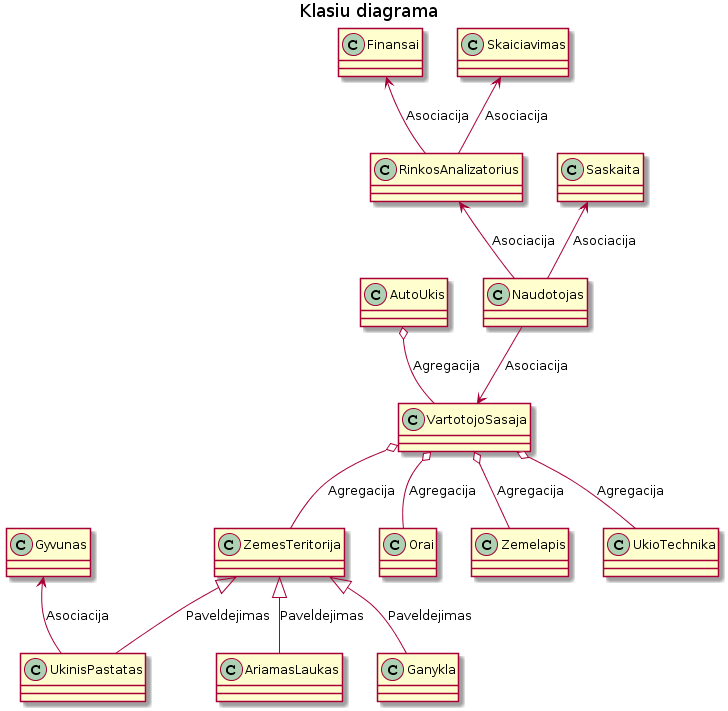
\includegraphics[width=18cm,height=17cm,keepaspectratio]{Klasesv2.png}
	\caption{}
	\label{fig:Klasesv2}
\end{figure}
	
	\begin{itemize}
		\item Dizainas:
			\begin{itemize}
				\item Visas programos dizainas(16 pav) paremtas Top to Bottom principu. Pradėjome galvoti dideliais objektais ir juos išskirstėm į mažesnius. Pagrindinė klasė yra AutoUkis, kuris iškviečia VartotojoSasaja klasę, kuri ir piešia visą prieinamumą vartotojams. Galima nesunkiai pridėti kitokią vartotojo sąsają ar bet kokią kitą UI piešimo galimybę, kaip, pavyzdžiui, piešti UI išmaniajame telefone. Programos modalumas leidžia nesunkiai pridėti funkionalumo, nes programos dalys yra atskiros viena nuo kitos. Pavyzdžiui, ištrynus klasę ŪkinisPastatas visos programos veikimas nesutriktų. 
			\end{itemize}
		\item Funkionalumas: 
			\begin{itemize}
				\item Programos funkcionalumas susideda iš trijų pagrindinių dalių, vartotojų prieiga prie sistemos, finansų bei išteklių (žmogiškųjų ir natūraliųjų) valdymas, išteklių sekimas. Prieigos dalyje funkcionalumas pasižymi prieigos išskaidymu - skirtingi sistemos vartotojai gauna skirtingą prieigą ir galimybes naudotis sistema. Pavyzdžiui, darbuotojas negali tvarkyti įmonės finansų, tačiau visi sistemos vartotojai gali kviesti greitąją pagalbą. Nesunku implementuoti naują vartotojų klasę (pvz. Svečias). Finansų bei išteklių dalyje ūkininkas gali tvarkyti savo išteklius, pavyzdžiui, samdyti arba atleisiti darbuotojus, stebėti rinkos kainą ir nuspręsti, kada jam palankiausia parduoti, sudarinėti sąskaitas ir tvarkyti kitą buhalteriją. Trečiojoje sistemos dalyje yra įgyvendinamas išteklių sekimas. Vartotojai, turintys prieigą gali stebėti žemės parametrus, ūkio technikos sąrašą, ūkinių pastatų sąrašą bei gyvūnų, priklausančių sistemai, sąrašą.
			\end{itemize}

	\end{itemize}

\pagebreak

\subsection{Kūrimo pjūvis}
	\begin{itemize}
		\item Dizainas:
		\begin{itemize}
			\item Programos dizainas stipriai paremtas Top to bottom projektavimo principu ir objektinio programavimo enkapsuliacijos paradigma. Sistema(18 pav) sukuria ir įgyvendina kitų sistemų intefeisus. Pagrindiniai keturi interfeisai, sukuriami programos, yra UkininkasUI, DarbuotojasUI ir AdminasUI, SOSPagalbaUI. Šie interfeisai suteikia prieigą prie sistemos skirtingas privilegijas turintiems vartojams. Sistema įgyvendina OruAPI kuriam interfeisą.

		\end{itemize}
	\end{itemize}

\begin{figure}[H]
		\centering	
	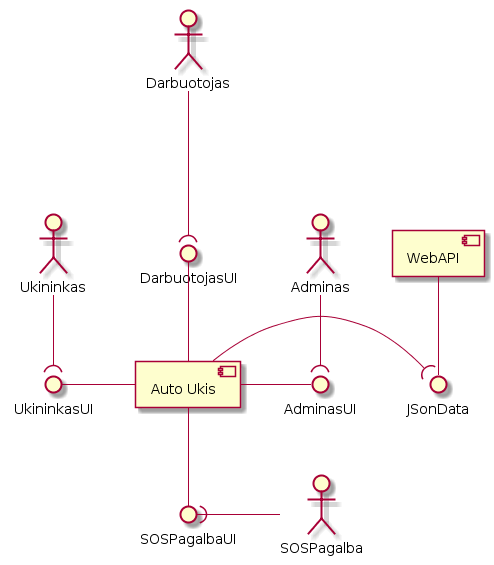
\includegraphics[width=17cm,height=20cm,keepaspectratio]{L0V2.png}
	\caption{}
	\label{fig:L0V2}
\end{figure}
	\begin{itemize}
	\item L0:
	\begin{itemize}
	\item Šioje diagramoje(18 pav) pavaizdavome sistemos bendradarbiavimą su išoriniais agentais, tokiais kaip MikroKontroleris, Ukininkas ir t.t. . Ši diagrama parodo sistemos įgyvendinamus ir kuriamus interfeisus. Iš diagramos matome, kad programos pagrindas kuria interfeisą ne tik vartotojams, bet ir tokiems išoriniams agentams, kaip SOS pagalba ir orų tarnyba.
\end{itemize}
	\begin{figure}[H]
		\centering	
	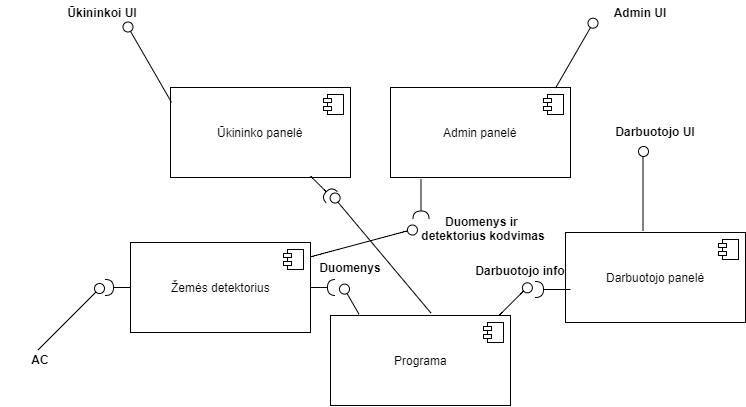
\includegraphics[width=17cm,height=20cm,keepaspectratio]{L1.png}
	\caption{L1 diagrama}
	\label{fig:L1}
\end{figure}
\item L1: Šioje diagramoje pavaizduotą, į kokius pagrindinius kompenentus išsiskaito visa programa. Iš diagramos matome, kad UI kontroleris, kuris kuria ir valdo vartotojo sąsajas išoriniams agentams, įgyvendina interfeisus kuriuos kuria komponentai žemėlapis, resursai ir ūkio technika, tai yra pagrindiniai programos komponentai, kuriuos papildo keletą kitų komponentų.

\end{itemize}
\pagebreak

\subsection{Use case}
Šiame skyriuje pavaizduoti visi galimai kuriuos gali atlikti atitinkamas programos vartotojas, use case diagrama padalinti į dvi dalis dėl patogumo skaitant.
\begin{itemize}
\item Diagramoje (26 pav) pavaizduoti veiksmai, kuriuos apdoroja komponentas resursai, bei kiti komponentai, kuria kuria interfeisus minėtajam.
		\begin{figure}[H]
		\centering	
	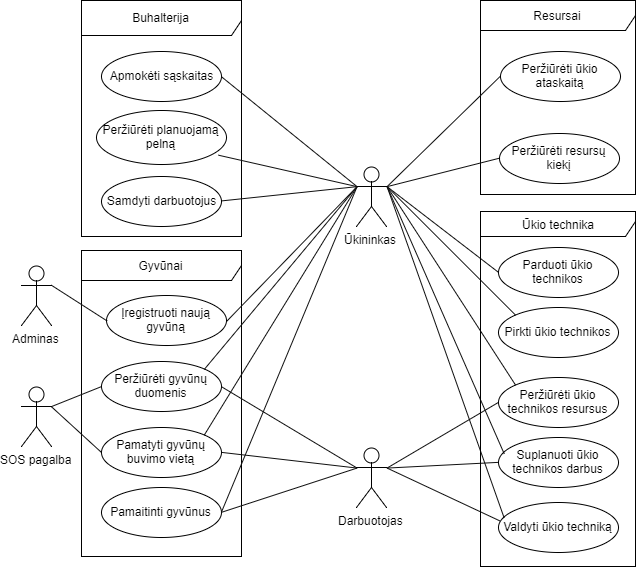
\includegraphics[width=15cm,height=17cm,keepaspectratio]{ResursaiUseCase.png}
	\caption{Use case. part 1}
	\label{fig:UseCaseFull}
\end{figure}
\item Šioje diagramoje pavaizduoti likusieji galimi veiksmai.
		\begin{figure}[H]
		\centering	
	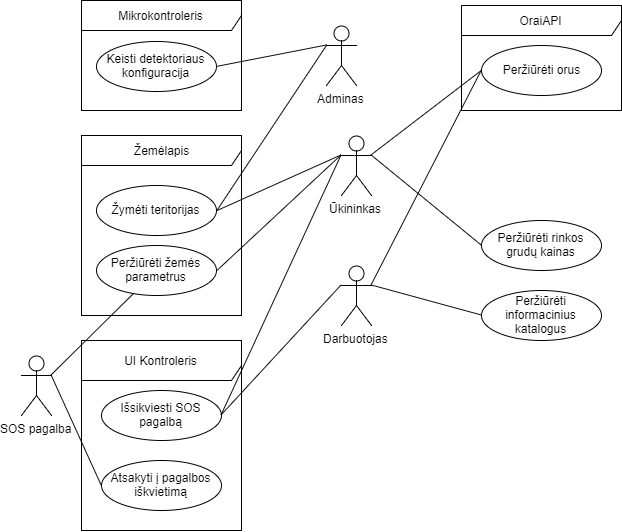
\includegraphics[width=15cm,height=17cm,keepaspectratio]{UseCase2.png}
	\caption{Use case. part 2}
	\label{fig:UseCaseFull}
\end{figure}
\end{itemize}
\begin{itemize}
		\item Elementų ir užduočių ryšių matrica:
\end{itemize}
\pagebreak

\subsection{Proceso pjūvis}
Šiame skyriuje pagrinde koncentruojamasi į programos elgseną jos vykdymo metu. Nurodomi pagrindiniai sistemos naudotojai ir jų atliekami veiksmai.
\subsubsection{Sekų diagramos}
\begin{itemize}
\item Diagramoje (6 pav)  pavaizduota seka, kurią programa atlieka Ukininkui norint gauti planuojamą jo pasirinkto laikotarpio pelną.
		\begin{figure}[H]
		\centering	
	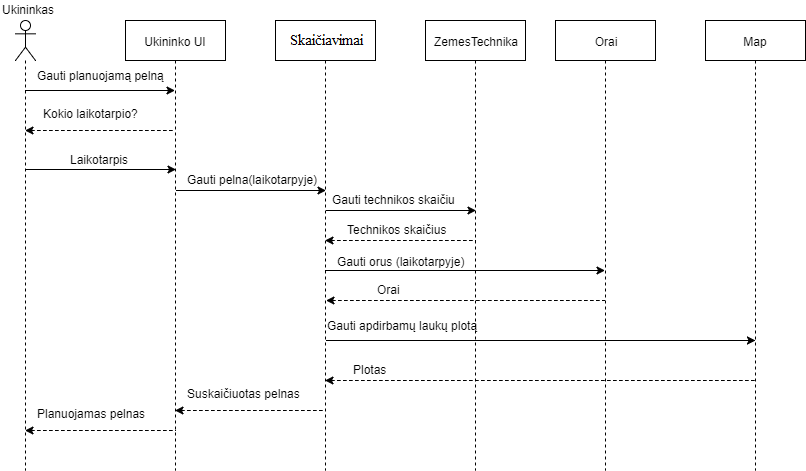
\includegraphics[width=17cm,height=20cm,keepaspectratio]{PelnoSkaičiavimas.png}
	\caption{}
	\label{fig:PelnoSkaičiavimas}
\end{figure}
Šioje diagramoje(6 pav) matome, kad ūkininkui pateikus užklausą planuojamui pelnui gauti, Ūkininkas UI kreipiasi į Skaičiavimai klasę su prašymu jį apskaičiuoti. Ši savo ruožtu norėdama gauti reikiamus duomenis kreipiasi į klases UkioTechnika, Žemėpalis ir Orai. Visi veiksmai atliekami vienas po kitos todėl neturėtų kilti ,,race" situacijos. Atlernatyviai būtų galimą į skaičiavimą įkelti gyvūnų biologinę statistiką(amžius, tikikmybė susirgti ligomis), bet tokia skaičiavimai būtų žymiai sudėtingesni.

\pagebreak

\item Teritorijos žimėjimo seka(7pav):
	\begin{figure}[H]
		\centering	
	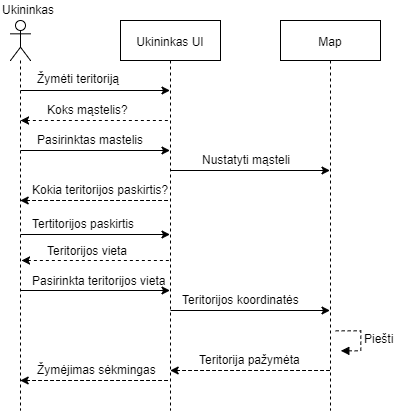
\includegraphics[width=10cm,height=10cm,keepaspectratio]{ŽymėtiTeritorijas.png}
	\caption{}
	\label{fig:ŽymėtiTeritorijas}
\end{figure}

Šioje diagramoje pavaizduotas veiksmų seka kurią atlieka sistema kai ūkininkas nori pažymėti kažkokią teritoriją žemėlapyje. Ūkininkas pasirinkimus padaro per Ukininkas UI ir ši klasė kreipiasi į Žemėlapis klasę. Alternatyviai būtų galima Žemėlapis klasę išskirstyti į kelias kitas klases dėl aiškumo.

\end{itemize}
\subsubsection{Būsenų diagramos}
\begin{itemize}
\item Detektoriaus būsenų diagrama(8 pav):

		\begin{figure}[H]
		\centering	
	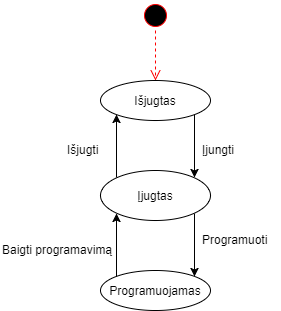
\includegraphics[width=7cm,height=7cm,keepaspectratio]{BusenuDetektorius.png}
	\caption{}
	\label{fig:BusenuDetektorius}
\end{figure}

\end{itemize}
Iš šios(29 pav) diagramos  matome, kad detektorius negali būt išjungtas programavimo metu, kad nekiltų klaidos vėlesnių paleidimų metu. Toks programos veikimas užtikriną, kad nebus prarandami kodo duomenys. 
\subsubsection{Veiklos diagramos}
\begin{itemize}
\item Orų sekimo veiklos diagrama(9 pav):
	\begin{figure}[H]
	\centering	
	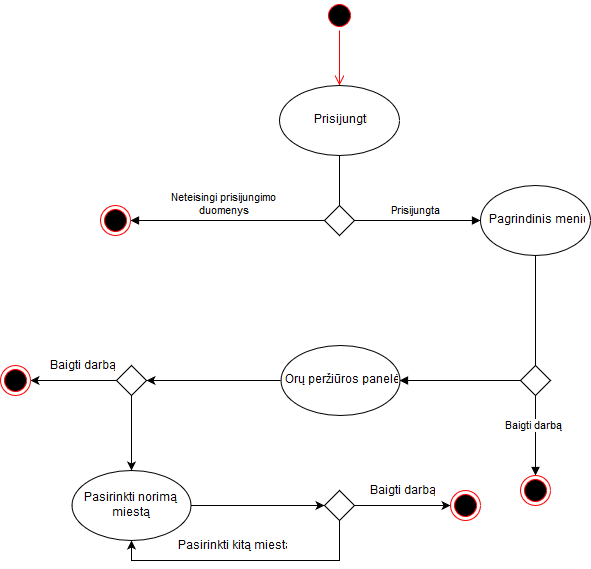
\includegraphics[width=10cm,height=10cm,keepaspectratio]{veiklos_diagrama_orai.png}
	\caption{}
	\label{}
	\end{figure}

Šioje diagramoje pavaizduotas programos vykdymo žingsniai norint peržiūrėti orus. Vartotojas negali patekti į pagrindinį meniu nesuvedęs teisingų prisijungimo duomenų. Pagrindiniame meniu vartotojas pasirenka orų stebėjimą. Tuomet sistema atidaro Orų peržūros langą kuriame vartotojas gali pasirinkti norimą miestą orų stebėjimui. betkuriuo metu po prisijungimo vartotojas turi galimybę baigti darbą.

\item Ūkio technikos sekimo veiklos diagrama(10 pav):
	\begin{figure}[H]
	\centering	
	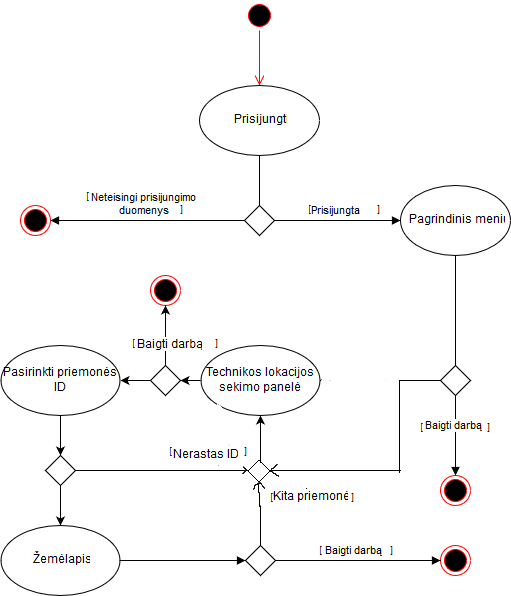
\includegraphics[width=10cm,height=10cm,keepaspectratio]{veiklos_diagrama_technikos_sekimas.png}
	\caption{}
	\label{}
	\end{figure}
Šioje pavaizduota kai programa veikia vartotojui norint naudotis ūkio technikos sekimo galimybe. Prieš pradedant darbą vartotojas turi prisijungti prie sistemos , kad galėtų pasinaudoti sistemos galimybėmis. Pagrindiniame sistemos lange psirenka technikos lokacijos sekimo galimybę ir sistema atidaro atitinkamą panelę. Iš ten vartotojas pasirenka technikos priemonės ID ir jeigu dėl kažkokių priežasčių sistemai nepavyksta rasti technikos priemonės vartotojas nukreipiamas atgal į technikos lokacijos sekimo panelę. Pavykus surasti technikos priemonę pagal jos ID vartotojui parodomas žemėlapis kuriame ir pademonstruota pasirinkta technikos priemonė. Iš žemėlapio vartotojas gali grįšti ir pasirinkti kitą transporto priemonę arba baigti darbą.
\pagebreak
\item Teritorijos žymėjimo veiklos diagrama(32 pav):
	\begin{figure}[H]
	\centering	
	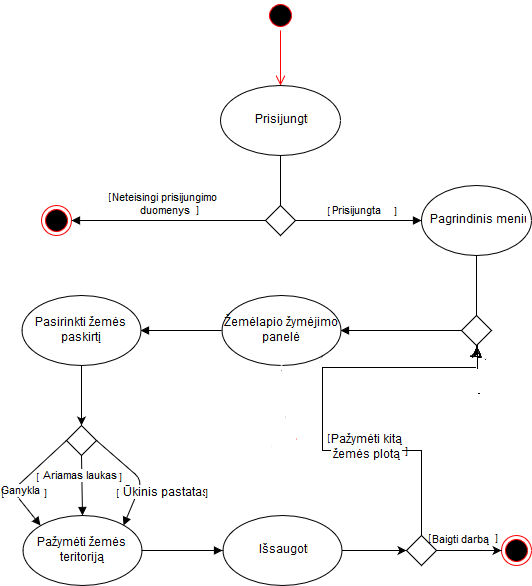
\includegraphics[width=10cm,height=10cm,keepaspectratio]{veiklos_diagrama_zymeti_teritorijas.png}
	\caption{}
	\label{}
	\end{figure}

Šioje diagramoje pavaizduotas sistemos veikimas vartotojui norint žymėti teritoriją. Norint pasinaudoti galimybę vartotojas turi prieijungti. Sėkmingai prisijungus vartotojas nukeliamas į pagrindinį programos meniu ir kurio gali pasirinkti žemėlapio žymėjimą. Pasirinkus žymėjima sistema atidaro Zemėlapio žymėjimo panelę kurioje vartotojas turi pasirinkti kokia yra norimos pažymėti žemės ploto paskirtis. Pasirinkus ploto paskirti vartotojas žemėlapyje pažymi žemės teritoriją ir išsaugo savo pažymėjimą. Po išsaugojimo vartotojas gali arba baigti darbą arba būti nukeltas į žymėjimo panelę ir žymėti žemėlapi toliau.
\item Gyvūnų suvedimo veiklos diagrama(12 pav):
	\begin{figure}[H]
	\centering	
	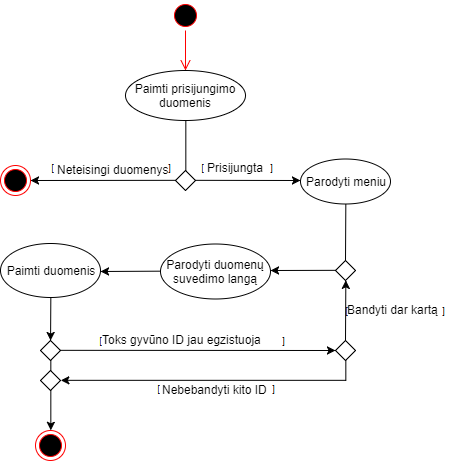
\includegraphics[width=10cm,height=10cm,keepaspectratio]{VeiklosGyvunuSuvedimas.png}
	\caption{}
	\label{}
	\end{figure}
\item Šiose diagramose matoma, kaip įgyvendinamas atitinkamas scenarijus programos vykdymo metu. Vartotojui norint pasinaudoti programos galimybėmis reikia įvesti teisingus prisijungimo duomenis. Tuomet vartotojas nukeliamas į pagrindinį parogramos meniu. Iš ten vartotojas pasirenka rodyti duomenų suvedimą. Sistema parodo gyvųnų duomenų langą ir tame pačiame lange vartotojas gali suvesti naujo gyvūno duomenis. Neteisingai suvedus duomenis varotojui duodamas pasirinkimas arba bandyti duomenis suvesti iš naudjo arba baigti darbą.
\end{itemize}
\subsection{Fizinis pjūvis}
	Šiame skyriuje parodoma programos naudojama aparatinė įranga, komunikacija tarp tinklo mazgų bei programos komponentų išdėstymas juose.
	\newline
	\vskip 0.5cm
	\begin{figure}[H]
	\centering	
	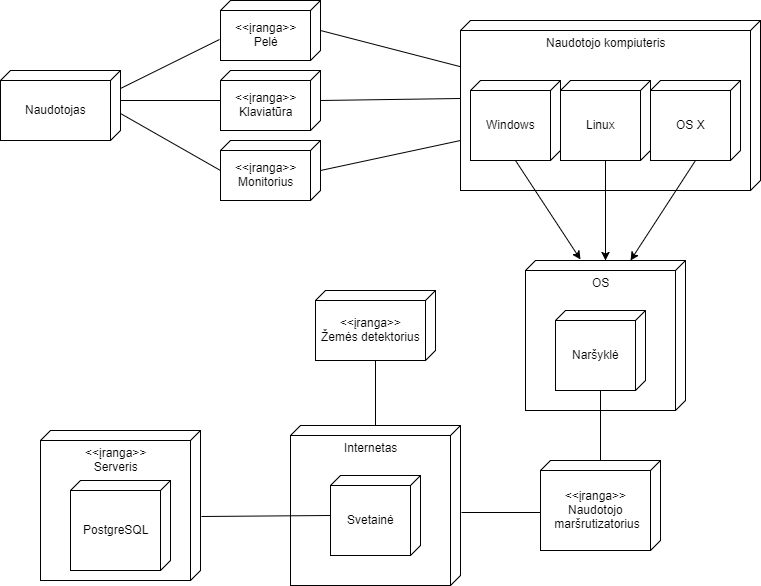
\includegraphics[width=15cm,height=15cm,keepaspectratio]{2D0.png}
	\caption{}
	\label{fig:Deployment}
\end{figure}
	\begin{itemize}
		\item D0: \hyperref[fig:Deployment]{\textit{Šioje diagramoje (34 pav.)}} parodyta, kaip išsaugomi programos duomenys. 
		Pirmoje projekto versijoje visi duomenys buvo saugomi kompiuteryje, vienintelis ryšys su internetu buvo per gismeteo.lt svetainę. Dabartinėje versijoje implementuotas duomenų saugojimas PostgreSQL duombazėje. Šioje diagramoje vaizduojamas kelias nuo naudotojo iki pasirinktos duombazės, naudojami techniniai įrenginiai ir jų sąryšiai su programinė įranga. Taip pat pridėtas žemės detektorius, kuris siunčia programai pasirinkto žemės ploto parametrų duomenis. Informacija, gauta iš žemės detektoriaus, taip pat talpinama PostgreSQL duombazėje.
	\end{itemize}

\pagebreak
\subsection{Antros dalies išvada}
Sistema suprojektuota tokiais principais, kad ją būtų lengva papildyti. Klasių dizainas atitinka Top->Bottom principą, kuris leidžia nesunkiai pridėti naujo funkcionalumo visai sistemai. Šis principas persikelia ir į kūrimo pjūvį. Sistemos įgyvendinami ir kuriami interfeisai yra labai moduliarūs ir nesunku pridėti ar išimti interfeisus iš sistemos. Vidinė programos struktūra sekų diagramoje aiškiai apibrėžia vartotojų sąveiką su sistema. Sekos išskirstytos diskrečiais ir aiškiais veiksmais, kas sumažina klaidų skaičių rašant kodą ir padeda suprasti, kaip viskas veikia. Iš fizinės pusės sistema yra serveryje ir dėl pasirinktos JAVA programavimo kalbos sistemą galimą pasileisti iš visų operacinių sistemų. Visa sistema yra serveryje. Duomenims saugoti psirinkome PostgreSQL, nes tai populiariausia nemokama duomenų bazių valdymo sistema. Sistemai yra vietos tobulėti. Ateityje egzistuoja galimybė ją pritaikyti išmaniesiams telefonams bei kitiems nešiojamiems įrenginiams.



\sectionnonum{Rezultatai ir išvados}
Projektuodami tą pačią sistemą du kartus skirtingais būdais pamatėme aiškius stilių skirumus. Kuriant sistemą nesilaikant jokių aiškių principų, kodas ir pati sistemos struktūra tampa neaiški, po kiek laiko prisimeni apie neįgyvendintus funkcionalumus arba idėjas, kurias įdėti į sistemą būtų labai sunku. Projektuojant sistemą antrą kartą buvo prisilaikyta Top->Bottom ir OOP principų, kurie leido lengviau struktūrizuoti visą darbą. Klasių ir komponentų diagramos pasidarė aiškiai suprantamos ir nauji funkcionalumai būtų nesunkiai įgyvendinami ateityje. Buvo aiškiau apibrėžtas fizinis sistemos principas, leidžiantis lanksciau naudotis sistema. Deja, ne viską pavyko pridėti. Norėtųsi įdėti išmaniojo telefono palaikymą mūsų sistemoje, bet dėl laiko stokos to nebepadarėme. Tačiau tikime, kad dėl struktūros pranašumų tai padaryti nebūtų sunku. Išmokome fundamentalius PSI aspektus, UML diagramų braižymą, išmokome naudotis keletu UML braižymo programų ir .pdf failų kurimo programa Latex, kuri palengvino darbą komandoje. Dėl gero darbų pasidalijimo projekto kūrimas vyko sklandžiai. 




\end{document}
